
\chapter{Fundamentação Teórica} \label{chap:FundamentacaoMatematica}

% Resumo opcional. Comentar se não usar.
\resumodocapitulo{Opcional, geralmente se colocam pequenos resumos
ou citações que se achar relevantes.}


\section{Introdução}

Este capítulo apresenta algumas soluções para o problema de tomada de decisões em sistemas de robótica móvel descritas em trabalhos anteriores nessa área. Ele aborda, também, o problema de aprendizagem por reforço e algumas alternativas relatadas na literatura. Por último, esse capítulo introduz a teoria matemática dos algoritmos utilizados nesse projeto.


\section{Revisão Bibliográfica} \label{section:RevisaoBibliografica}

Aqui são descritas diferentes abordagens encontradas na literatura para o problema de tomada de decisões aplicado a sistemas de robótica móvel. A tomada de decisões é um problema de amplo espectro para o qual existem várias estratégias diferentes de solução.

Analisando a literatura recente, é possível ver a preferência crescente por algoritmos probabilísticos nessa área, no lugar dos determinísticos. Para uma modelagem realista do ambiente do robô, é preciso considerar as incertezas nele presentes.

Muitos algoritmos de planejamento de tarefas são específicos para as tarefas que os robôs desempenham. Alguns exemplos são na área de exploração, por exemplo, o uso de algoritmos de exploração de fronteiras \cite{conf:icra:FredaO05,Yamauchi:1998:FEU,Yamauchi:1997:FAA}, ou na área de braços robóticos, para manipulação de objetos \cite{Berenson_2009_6465}.

Neste trabalho, é desejado um algoritmo que não seja específico para um único tipo de aplicação. Ao analisar a literatura recente, vê-se que muitos algoritmos nessa área são baseados em cadeias de Markov. Essa teoria assume que um ambiente pode ser modelado por um certo número de variáveis de estados e que cada estado depende apenas do estado anterior, ou seja, o sistema não tem memória de longo prazo \cite{books:daglib:0095301}.
\begin{equation}
	P(S^t\mid S^{t-1}S^{t-2})=P(S^t\mid S^{t-1})
\end{equation}

Um algoritmo frequentemente utilizado baseado em cadeias de Markov é o Processos de Decisão de Markov (Markov Decision Processes, MDP) \cite{Thrun:2005:PR:1121596}. Embora o MDP leve em conta que as ações executadas possam ter um resultado imprevisível, ele não incorpora a incerteza provinda dos sensores. Em outras palavras, ele considera que os estados do sistema podem ser completamente observados a todo instante, o que, em robótica, não é o caso.

Um algoritmo de extensão do MDP que corrige esse problema é o Processos de Decisão de Markov Parcialmente Observável (Partially Observable Markov Decision Processes, POMDP) \cite{Thrun:2005:PR:1121596}. Esse algoritmo retorna para o caso geral completamente probabilístico em que tanto sensores quanto atuadores tem funcionamento imprevisível e com certa curva conhecida de probabilidade. O problema com esse algoritmo é a sua demanda computacional, mesmo podendo ser calculado \textit{offline} e salvo, ele muitas vezes não é computacionalmente aceitável.

Pineau e Thrun \cite{Pineau01hierarchicalpomdp} utilizam uma estratégia de vários POMDPs hierarquizados para reduzir o problema de esforço computacional que um único POMDP combinado iria precisar. Embora a demanda computacional seja reduzida com essa estratégia, dependendo do tamanho do espaço de estados, ela ainda não é tolerável.

Outra estratégia para o planejamento de tarefas é a abordagem bayesiana para seleção de comportamentos presente em \cite{Koike:2005,lidoris2008}. Essa é uma estratégia interessante por ser computacionalmente eficiente, pois, ao selecionar somente um comportamento e posteriormente escolher uma ação para ele, consegue reduzir consideravelmente as opções possíveis (existem menos comportamentos do que ações possíveis). Essa estratégia foi expandida posteriormente em \cite{lidoris2011state}, onde são aprendidos os modelos probabilísticos de seleção de comportamentos a partir de entradas humanas.

Na área de aprendizagem de modelos ou de políticas para execução de ações, existem vários algoritmos baseados no MDP citado acima. Alguns deles focam apenas na aprendizagem do modelo \cite{calvet:hal-00674226,Gutmann_noise-contrastiveestimation} e tem várias aplicações, sendo análise de mercados uma delas \cite{calvet:hal-00674226}. Outro exemplo de algoritmo de aprendizagem é o de diferença temporal, que é utilizado para avaliar uma dada política%
\footnote{Uma política pode ser vista como uma função $ \pi \left( S \right) $, a qual, dado um estado, retorna uma ação possível de ser executada nele.%
}
\cite{Sutton:1988:LPM,Andreas:2007,sutton1998reinforcement}.

Outras estratégias de aprendizagem por reforço permitem aprender uma política ótima de comportamentos ou ações para um dado agente. Uma delas é o \textit{Q Learning} \cite{sutton1998reinforcement,KLMSurvey}, que é um algoritmo simples, mas eficiente, que aprende valores de ganho para cada par ação-estado, e com isso consegue alcançar uma política ótima. Outro algoritmo relevante é o ator crítico \cite{sutton1998reinforcement,RicAbeYu07,conf:nips:BhatnagarSGL07,Konda01actor-criticalgorithms}, que aprende uma política ótima ao separar um ator, que escolhe e executa essa política, e um crítico, que avalia a política e provê feedback para o ator.

Nesse trabalho, uma abordagem é apresentada, baseada em \cite{Koike:2005,lidoris2008}, para fazer a seleção de comportamento e de ação de um agente móvel com sensores probabilísticos. Além disso, um algoritmo de aprendizagem por reforço, \textit{Q Learning}, é utilizado para aprender uma política ótima de escolha de comportamento, presente em \cite{sutton1998reinforcement}.


\section{Filtro Bayesiano} \label{section:FiltroBayesiano}

Um filtro bayesiano é uma abordagem probabilística. Ele estima uma função de densidade de probabilidade desconhecida de forma recursiva no tempo, utilizando ações e observações, além de um modelo matemático do processo.

No filtro bayesiano é desejado estimar a distribuição conjunta de probabilidade:
\begin{equation} \label{equation:DistribuicaoConjuntaProbabilistica}
	P ( M^{0: t} S^{0: t} Z^{0: t} \mid \pi_f ),
\end{equation}
sendo $ M^i $ o conjunto de ações, $ S^i $ o estado do sistema, $ Z^i $ os dados dos sensores, todos nesse instante i, e $ t $ o instante de tempo para o qual se deseja obter o valor dessa distribuição. Essa função de probabilidade representa a probabilidade de uma sequência de ações, observações e estados acontecerem dado o que se sabe sobre o mundo ($ \pi_f $). Para obter essa distribuição assume-se que esse sistema pode ser modelado como na distribuição conjunta presente na equação \ref{equation:FiltroBayesiano1}.

\begin{equation} \label{equation:FiltroBayesiano1}
        P ( M^{0: t} S^{0: t} Z^{0: t} \mid \pi_f ) = P ( M^0 S^0 Z^0 \mid \pi_f ) \cdot \prod\limits_{j =1}^{t} 
        \left(
            \begin{array}{l}
                P( S^j \mid S^{j -1} M^{j -1} \pi_f ) \\
                \times P( Z^j \mid S^j \pi_f ) \\
                \times P( M^j \mid S^j M^{j -1} \pi_f )
            \end{array}
        \right).
\end{equation}

Essa equação explicita quatro itens:

\begin{itemize}
  \item $ P \left( M^0 S^0 Z^0 \mid \pi_f \right) $ : As probabilidades do estado inicial do sistema são necessárias para se obter seus futuros valores;
  \item $ P \left( S^j \mid S^{j-1} M^{j-1} \pi_f \right) $ : Cada estado depende do estado anterior e da ação tomada no tempo anterior (modelo de movimento);
  \item $ P \left( Z^j \mid S^j \pi_f \right) $ : É necessário um modelo probabilístico do sensor. Esse termo representa a probabilidade de se ter recebido uma certa medida dos sensores, dado que o estado atual realmente seja $ S^j $ (modelo de observação);
  \item $ P \left( M^j \mid S^j M^{j-1} \pi_f \right) $ : A escolha da próxima ação depende de qual o estado do sistema e qual foi a ação anterior (modelo de ação motora).
\end{itemize}

\begin{figure}[h]
    \centering
    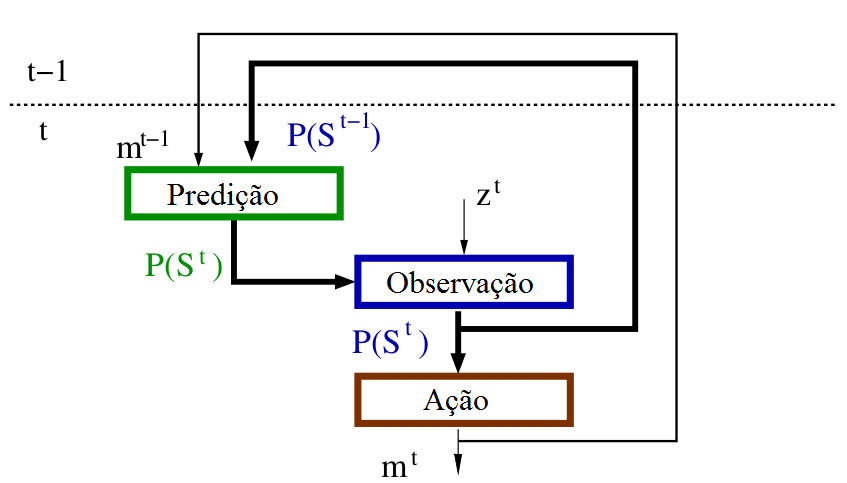
\includegraphics[width=120mm]{images/modelo_bayesiano-carla}
    \caption{\label{img:ModeloProbabilisticoCarla}Filtro Bayesiano Recursivo. Fonte: \cite{Koike:2005}}
\end{figure}

A partir dessas densidades probabilísticas, pode-se decidir por uma estratégia de ação em qualquer instante de tempo utilizando a ação $ M^t = m $ que maximize a função \ref{equation:FiltroBayesiano1}. Pode-se também descobrir o estado mais provável do sistema num instante de tempo $ j $, calculando essa distribuição (equação \ref{equation:FiltroBayesiano1}) e vendo qual estado $ s^j \in S^j $ possui maior probabilidade.

Esse modelo pode, ainda, ser discretizado para cada instante de tempo, sendo descrito pela equação \ref{equation:FiltroBayesiano1Recursivo}.

\begin{equation} \label{equation:FiltroBayesiano1Recursivo}
        P ( M^{0: t} S^{0: t} Z^{0: t} \mid \pi_f ) = P ( M^{0: t-1} S^{0: t-1} Z^{0: t-1} \mid \pi_f ) \cdot 
        \left(
            \begin{array}{l}
                P( S^t \mid S^{t -1} M^{t -1} \pi_f ) \\
                \times P( Z^t \mid S^t \pi_f ) \\
                \times P( M^t \mid S^t M^{t -1} \pi_f )
            \end{array}
        \right).
\end{equation}

Com isso tem-se um modelo recursivo que pode ser utilizado a cada instante de tempo para atualizar o modelo de probabilidades. Essa atualização pode ainda ser dividida em três partes distintas: predição, observação e escolha de ação motora.

\subsection{Predição}

Nessa etapa, a partir da ação escolhida e executada no período anterior de tempo (instante de tempo $ t-1 $), é realizada uma estimativa de qual será o estado após sua execução (instante de tempo $ t $).

\begin{equation}
    P \left( S^t \mid z^{0: t-1} m^{0: t-1} \pi_f \right) \propto \sum\limits_{S^{t-1}}
        \left(
            \begin{array}{l}
                P \left( S^t \mid S^{t-1} m^{t-1} \pi_f \right) \\
                \times P \left( m^{t-1} \mid S^{t-1} m^{t-2} \pi_f \right)\\
                \times P \left( S^{t-1} \mid z^{0: t-1} m^{0: t-2} \pi_f \right)
            \end{array}
        \right).
\end{equation}


\subsection{Observação}

Então, o estado probabilístico (\textit{belief state}) do agente é atualizado a partir dos sensores presentes no robô.

\begin{equation}
    P \left( S^t \mid z^{0: t} m^{0: t-1} \pi_f \right) \propto 
        \left(
            \begin{array}{l}
                P \left( z^t \mid S^t \pi_f \right) \\
                \times P \left( S^t \mid z^{0: t-1} m^{0: t-1} \pi_f \right)
            \end{array}
        \right).
\end{equation}


\subsection{Escolha de ação motora}

Por último, a seleção de uma ação a ser executada pelo robô é realizada. Calcula-se a distribuição de probabilidade de cada ação $ m^t \in M^t $ e aquela com maior valor de probabilidade é escolhida.

\begin{equation}
    P \left( M^t \mid z^{0: t} m^{0: t-1} \pi_f \right) \propto \sum\limits_{S_i^t}
        \left(
            \begin{array}{l}
                P \left( M^t \mid S^t m^{t-1} \pi_f \right)\\
                \times P \left( S^t \mid z^{0: t} m^{0: t-1} \pi_f \right)
            \end{array}
        \right).
\end{equation}


\section{MDP (Processo de Decisão de Markov)} \label{section:MDP}

MDPs são utilizados em várias áreas, como: economia, manufatura de processos e robótica. Ele foi nomeado a partir de Andrey Markov e provê uma base matemática para o modelamento de tomada de decisões. Eles são uma extensão de cadeias de Markov, tendo como diferença a adição de ações e recompensas (escolha e motivação).

MDP é, mais precisamente, um processo de controle estocástico de tempo discreto. Isso significa que ele é um processo de controle probabilístico, baseado em passos (\textit{time steps}). Em cada passo o robô se encontra em um estado $ S $ perfeitamente conhecido em que pode-se executar qualquer ação $ u $ disponível para esse estado. O modelo de percepção do robô, $ p \left( Z \mid S \right) $ é uma equação determinística e bijetora, o robô só pode estar em um estado $ s \in S $ para uma percepção $ z \in Z $ do ambiente.

Após executada essa ação, o robô se encontra em um novo estado $ s' \in S $ com probabilidade $ p \left( s' \mid u, s \right) $, essa equação é conhecida como modelo de atuação (\textit{action model}). O modelo de atuação não é, em geral, determinístico, ou seja, uma ação pode ter várias consequências com diferentes probabilidades. Uma consequência disso é que planejar uma única sequência de ações não é o suficiente, o planejador deve decidir por uma ação para cada possível estado $ s \in S $, em que o robô possa se encontrar.

No grafo da figura \ref{img:MapaDeProbabilidadesMarkov}, para uma ação A ou B, tem-se indicadas as probabilidades $ p \left( s' \mid u, s \right) $ através do percentual indicado nas setas saindo do estado $ s $ para $ s' $. Pode-se ver que, para esse sistema, $ P \left( s2 \mid a, s1 \right) = 0.2 $ e $ P \left( s4 \mid a, s1 \right) = 0.8 $. Se $ s1 $ for o estado inicial e $ s6 $ for o objetivo, não adianta obter uma sequência de ações $ a \rightarrow a \rightarrow b$, por exemplo, pois seria possível que o robô se encontrasse em vários possíveis estados ao final dessa sequência: $ s4 $, $ s2 $ ou $ s6 $.

\begin{figure}[h]
    \centering
    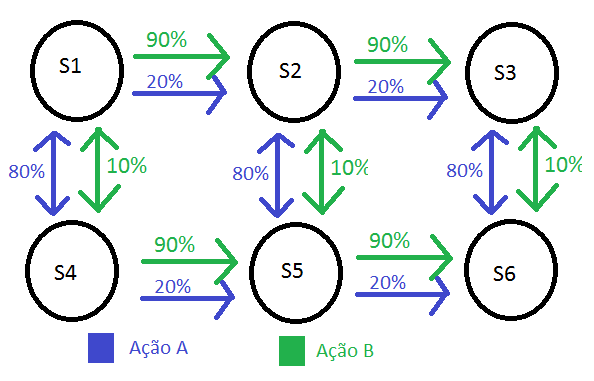
\includegraphics[width=120mm]{images/probabilidade-markov}
    \caption{Mapa de Probabilidades}
    \label{img:MapaDeProbabilidadesMarkov}
\end{figure}

É necessário mapear uma ação para cada estado possível, gerando o que é chamado de política de controle (\textit{control policy}). Essa política de controle tem formato $ \pi: S^t \rightarrow U^t $, ou seja, a política $ \pi $ recebe um estado $ s^t $ e retorna a ação $ u^t $ planejada para ele. Portanto, com a política $ \pi \left( S \right) $, não há mais o problema anterior, pois o planejamento da ação a cada instante é baseado no estado em que o robô se encontra.

Calcular essa política não é trivial, devido, principalmente, à existência de infinitos caminhos para se chegar de um estado $ s1 $ a $ s6 $. Um possível caminho é $ s1 \rightarrow s2 \rightarrow s3 \rightarrow s6 $, por exemplo, outro caminho seria $ s1 \rightarrow s2 \rightarrow s5 \rightarrow s2 \rightarrow s3 \rightarrow s6 $, e outro ainda é $ s1 \rightarrow s2 \rightarrow s5 \rightarrow s2 \rightarrow s5 \rightarrow s2 \rightarrow s3 \rightarrow s6 $.

Antes de obter um algoritmo definitivo, é necessário modelar o objetivo do problema. Para isso é utilizada uma função de recompensa para o robô $ r \left( S, U, S' \right) $ que retorna um número real. Ela indica quão desejado é se chegar a um estado $ s' \in S' $ a partir de $ s \in S $ executando a ação $ u \in U $. Para sistemas cujo único objetivo é chegar a estados desejados, é possível simplificar essa função para $ r \left( s' \right) $, por exemplo.

Sabendo que é desejado encontrar uma política que maximize o ganho de recompensas, é possível gerar um plano de políticas ótimo pensando-se apenas na próxima ação, maximizando uma recompensa imediata. Caso as recompensas sejam dadas apenas pela escolha de uma ação baseada no estado atual $ r \left( S, U \right) $, sem considerar o estado alcançado, uma possível escolha de política seria a dada pela equação \ref{equation:policySelectionMDP1Step}.

\begin{equation} \label{equation:policySelectionMDP1Step}
    \pi_1 \left( s \right) = \underset{u}{argmax} \left( r \left( s, u \right) \right).
\end{equation}

Como a recompensa depende também do estado alcançado, é necessário ponderar cada recompensa $ r \left( S, U, S' \right) $ pela probabilidade de se alcançar um estado $ s' \in S' $:

\begin{equation}
    \pi_1 \left( s \right) = \underset{u}{argmax} \left( \int \! r \left( s, u, s' \right) \cdot P \left( s' \mid u, s \right) \, \mathrm{d}s' \right).
\end{equation}

É possível então gerar, para essa política, uma função de valor (\textit{value function}) que representa a recompensa esperada para cada estado $ s $ seguindo a política $ \pi $:

\begin{equation}
    V_1 \left( s \right) = \underset{u}{max} \left( \int \! r \left( s, u, s' \right) \cdot P \left( s' \mid u, s \right) \, \mathrm{d}s' \right).
\end{equation}

Ao pensar dois passos a frente, pode-se utilizar esse novo valor $ V_1 \left( S \right) $ para calcular a política, planejando agora um passo à frente de antes. Depois generaliza-se esse pensamento para qualquer caso futuro, pensando $ j $ passos a frente.

\begin{equation}
    \pi_j \left( s \right) = \underset{u}{argmax} \left( \int \! \left( r \left( s, u, s' \right) + \gamma \cdot V_{j-1} \left( s' \right) \right) \cdot P \left( s' \mid u, s \right) \, \mathrm{d}s' \right).
\end{equation}

Onde $ \gamma $ é uma constante de desconto, usada para incentivar o ganho de recompensas imediatas em oposição às tardias. Essa função indica que a política ótima é a que gera uma maior recompensa imediata, somada com a somatória de todas as recompensas futuras esperadas, ponderadas pelas probabilidades de serem recebidas. Gera-se, novamente, uma função de valor para essa política, presente na equação \ref{equation:ValueFunctionTimeT}.

\begin{equation} \label{equation:ValueFunctionTimeT}
    V_j \left( s \right) = \underset{u}{max} \left( \int \! \left( r \left( s, u, s' \right) + \gamma \cdot V_{j-1} \left( s' \right) \right) \cdot P \left( s' \mid u, s \right) \, \mathrm{d}s' \right).
\end{equation}

Ao pensar $ j = \infty $ passos à frente, a política geralmente converge e uma política ótima para esse sistema é encontrada.

\begin{equation}
    \pi^* \left( s \right) = \pi_\infty \left( s \right) = \underset{u}{argmax} \left( \int \! \left( r \left( s, u, s' \right) + \gamma \cdot V_\infty \left( s' \right) \right) \cdot P \left( s' \mid u, s \right) \, \mathrm{d}s' \right).
\end{equation}

\begin{equation} \label{equation:ValueFunctionMDP}
    V^* \left( s \right) = V_\infty \left( s \right) = \underset{u}{max} \left( \int \! \left( r \left( s, u, s' \right) + \gamma \cdot V_\infty \left( s' \right) \right) \cdot P \left( s' \mid u, s \right) \, \mathrm{d}s' \right).
\end{equation}


\section{TD (Diferença Temporal)} \label{section:TD}

Caso não se conheçam os valores das recompensas $ r \left( S, U, S' \right) $ e nem resultado de uma ação $ P \left( s' \mid u, s \right) $ pode-se utilizar, como solução, a aprendizagem de reforço. O algoritmo de diferença temporal visa, a partir de uma política fixa $ \pi \left( S \right) $, aprender os valores finais de $ V \left( S \right) $ através da execução de ações em diferentes estados, sem ter um conhecimento prévio das recompensas recebidas ou do modelo probabilístico do resultado de suas ações.

Esse algoritmo baseia-se na equação \ref{equation:ValueFunctionMDP} obtida no seção \ref{section:MDP} e parte da premissa de que uma política $ \pi_{td} $ já foi escolhida. Ele então atualiza o valor de $ V \left( S \right) $ a cada experiência qualquer $ \left( s, u, s', r \right) $, ou seja, sempre que um estado $ s' \in S $ é alcançado a partir do estado $ s \in S $, com uma ação $ u \in U $ e recebendo uma recompensa $ r \in \mathbb{R} $. A partir de cada dessas experiências, pode-se obter um valor $ amostra $ tal que:

\begin{equation} \label{equation:AmostraTD}
	amostra = r \left( s, u, s' \right) + \gamma \cdot V_{\pi_{td}}^t \left( s' \right).
\end{equation}

Agora, escolhendo-se uma constante de aprendizagem $ \alpha $, pode-se atualizar o valor de $ V_{\pi_{td}} \left( s \right) $ tal que:

\begin{equation} \label{equation:UpdateValueFunctionTD}
	V_{\pi_{td}}^t \left( s \right) = \left( 1 - \alpha \right) \cdot V_{\pi_{td}}^{t-1} \left( s \right) + \alpha \cdot amostra.
\end{equation}

É possível observar que, utilizando valores suficientemente pequenos de $ \alpha $, os valores de $ V_{\pi_{td}} \left( s \right) $ convergem com o tempo e, principalmente, convergem para os mesmos valores que o algoritmo MDP, considerando que a política $ \pi_{td} $ utilizada é ótima.

A limitação da diferença temporal é que ela apenas avalia uma política fixa já existente. Caso deseje-se mudar a política, ou gerar uma utilizando este algorítmo, surge um problema, pois todos os valores de $ V \left( S \right) $ dependem somente do estado e não da ação executada. Caso a política $ \pi_{td} $ executada seja alterada, é necessário recalcular todos os valores $ V \left( S \right) $.

\section{Q Learning} \label{section:QLearning}

\textit{Q Learning} é um dos mais conhecidos e mais utilizados algoritmos de aprendizagem por reforço, sendo utilizado para controle de robôs \cite{Gaskett:2002}, tratamento de problemas em processamento de imagens \cite{Alexandru-Learning} e criação de sistemas de troca financeiros \cite{RePEc:ven:wpaper:2014:15}. Esse é um algoritmo de aprendizagem ativa, ou seja, a escolha da política e das ações é feita juntamente com a aprendizagem e é possível alcançar uma nova política ótima.

Ao invés de utilizar o valor de $ V \left( S \right) $, na equação \ref{equation:ValueFunctionMDP}, o \textit{q learning} utiliza um valor $ Q \left( S, U \right) $, tal que:
\begin{equation} \label{equation:PolicySelectionQLearning}
    \pi^t \left( s \right) = \underset{u}{argmax} \left( Q^t \left( s, u \right) \right), e
\end{equation}

\begin{equation}
    V^t \left( s \right) = \underset{u}{max} \left( Q^t \left( s, u \right) \right).
\end{equation}

Ou seja:
\begin{equation} \label{equation:QValueFunctionQLearning}
    Q^t \left( s, u \right) = \int \! \left( r \left( s, u, s' \right) + \gamma \cdot V^{t-1} \left( s' \right) \right) \cdot P \left( s' \mid u, s \right) \, \mathrm{d}s',
\end{equation}
que pode ser reescrito como:
\begin{equation} \label{equation:QValueFunctionQLearningFinal}
    Q^t \left( s, u \right) = \int \! \left( r \left( s, u, s' \right) + \gamma \cdot \underset{u'}{max} \left( Q^{t-1} \left( s', u' \right) \right) \right) \cdot P \left( s' \mid u, s \right) \, \mathrm{d}s'.
\end{equation}

Ao aprender o valor de $ Q^t \left( S, U \right) $, ao invés do de $ V^t \left( S \right) $, é possíver modificar a política sem ter de reaprender todos os seus valores. Analogamente às equações \ref{equation:AmostraTD} e \ref{equation:UpdateValueFunctionTD} em TD, aprende-se através de amostras obtidas a partir de experiências $ \left( s, u, s', r \right) $:
\begin{equation} \label{equation:AmostraQLearning}
	amostra = r \left( s, u, s' \right) + \gamma \cdot \underset{u}{max} \left( Q^{t-1} \left( s', u' \right) \right), e
\end{equation}

\begin{equation} \label{equation:QUpdateQLearning}
	Q^t \left( s, u \right) = \left( 1 - \alpha \right) \cdot Q^{t-1} \left( s, u \right) + \alpha \cdot amostra.
\end{equation}

Com um número suficiente de iterações e um decaimento apropriado do parâmetro de aprendizagem $ \alpha $, $ Q^t \left( S, U \right) $ tende a um valor ótimo  com uma probabilidade 1 \cite{journals:ml:Tsitsiklis94,Jaakkola94convergenceof,Watkins:1989} e a política escolhida com base na função \ref{equation:PolicySelectionQLearning} também é ótima.

Algumas limitações com esse algoritmo são:

\begin{itemize}
	\item Podem existir muitos estados para se visitar: em um espaço contínuo, por exemplo, seriam infinitos;
	\item Podem existir muitas ações possíveis para cada estado: para o acionamento analógico de um motor, por exemplo, seriam infinitas;
	\item Se houverem muitos pares ação-estado $ \left( S, U \right) $, mesmo que seja possível aprender por um tempo muito grande, é necessário armazenar o valor de $ Q^t \left( S, U \right) $ para cada ação que for possível de ser executada em cada estado;
	\item O algoritmo não consegue aplicar o que aprendeu em um estado para outros estados com características similares.
\end{itemize}

\subsection{Generalização dos Pares Estado-Ação} \label{subsection:GeneralizaçãoParesEstadoAção}

Uma solução para esses problemas é generalizar a informação de um par estado-ação para outros similares. Para isso utiliza-se um vetor de características $ f $ para descrever o estado. Essas características podem ser:

\begin{itemize}
	\item Distância para uma posição que oferece uma recompensa positiva;
	\item Distância para uma posição que oferece uma recompensa negativa;
	\item Número de alvos a serem capturados;
	\item Estado do robô (Com ou sem defeito).
\end{itemize}

Elas também podem descrever a ação a ser executada, como:

\begin{itemize}
	\item Ficar parado;
	\item Mover uma garra;
	\item Economizar energia.
\end{itemize}

Essas características podem, também, descrever um estado futuro $ s' $ (possivelmente utilizando alguma das características descritas acima) que tenha grande chance de ser alcançado por esse par estado-ação.

Utiliza-se esse vetor $ f $ de características $ f_j \left( S, U \right) $ para obter um valor $ Q \left( S, U \right) $ tal como descrito na equação \ref{equation:QValueGeneralizado}.

\begin{equation} \label{equation:QValueGeneralizado}
	Q \left( S, U \right) = \omega_1 \cdot f_1 \left( S, U \right) + \omega_2 \cdot f_2 \left( S, U \right) + \cdots + \omega_n \cdot f_n \left( S, U \right).
\end{equation}

Sendo $ \omega_j $ um peso, que é o que se quer aprender nesse algoritmo, utilizado para ponderar o valor de cada característica $ f_j $. Com essa equação se consegue um valor parecido de $ Q \left( S, U \right) $ para estados distintos, mas que possuam características $ f_j \left( S, U \right) $ com valores parecidos. A desvantagem é que deve-se escolher esses valores/características com cuidado para obter uma boa representação do par estado-ação a partir deles, ou pode-se obter estados-ações com valores de $ f_j \left( S, U \right)$ parecidos, e, consequentemente, valores de $ Q \left( S, U \right) $ também parecidos, mas que são muito diferentes na aplicação.

Com esse novo modelo, aprende-se valores a partir de cada experiência, utilizando o erro atual do modelo, descrito pela equação \ref{equation:ErrorFunctionQLearning1}.

\begin{equation} \label{equation:ErrorFunctionQLearning1}
	erro = r \left( s, u, s' \right) + \gamma \cdot \underset{u}{max} \left( Q^{t-1} \left( s', u' \right) \right) - Q^{t-1} \left( s, u \right).
\end{equation}

Esse erro é calculado pela diferença entre a recompensa recebida, somada com o valor de ganho esperado para o novo estado alcançado e o valor atual esperado para o par estado-ação executada. Utiliza-se o erro acima para atualizar cada um dos pesos usados para obter $ Q_t \left( S, U \right) $, como explicitado na equação \ref{equation:OmegaUpdate1}.

\begin{equation} \label{equation:OmegaUpdate1}
	\omega_i^t = \omega_i^{t-1} + \alpha \cdot erro \cdot f_i \left( s, u \right)
\end{equation}

Assim, caso haja um erro grande para um dado estado, os valores de todos os estados com características similares àquele são atualizados. É importante notar também que, caso esse estado tenha um valor maior para uma característica $ f_j $, o peso $ \omega_j $ dela terá maior alteração que os das outras características.

A função utilizada para calcular $ Q \left( S, U \right) $ é um perceptron%
\footnote{Um perceptron é um algoritmo de apredizagem supervisionada para classificar uma entrada em uma de várias opções. Ele é um classificador linear, ou seja, ele utiliza uma série de pesos, combinados com um vetor de características, para fazer essa classificação.%
} e esse tipo de função possui limitações, sendo a principal delas a capacidade de aprender apenas problemas linearmente separáveis \cite{Haykin:1998:NNC:521706,priddy2005artificial}. Por isso, os parâmetros $ f_i \left( S, U \right) $ devem ser bem escolhidos: não só para caracterizar bem um estado e permitir uma boa diferenciação entre dois deles, mas também para permitir essa aprendizagem.

\subsection{Escolha de Ações e Exploração Gulosa} \label{subsection:EscolhaDeAçõesExploraçãoGulosa}

Utilizando a equação \ref{equation:PolicySelectionQLearning}, em conjunto com \ref{equation:QValueGeneralizado}, é possível criar uma política $ \pi $ para escolha de ações. Essa política, caso o valor de $ Q \left( S, U \right) $ já tenha sido aprendido com sucesso, será ótima.

Mas, se desde o começo do aprendizado esse método for utilizado para escolher a ação executada, é possível ficar preso em máximas locais%
\footnote{Uma política de ação que é melhor do que outras com pequenas variações, mas, caso se mude mais os parâmetros, existem outras melhores.%
}, sem explorar outras opções de ação. Um meio de evitar esse problema é utilizar outros métodos de exploração durante o treinamento, que podem ser desativados quando o treinamento acabar. 

Um desses métodos é chamado de exploração gulosa (\textit{greedy exploration}). É um método em que, antes de se selecionar uma ação, se ``arremessa uma moeda'': dependendo do resultado, ou uma ação randômica é executada, ou uma ação baseado nos valores de $ Q^t \left( S, U \right) $ atuais é escolhida, sendo escolhida a ação que maximize o valor dessa função $ Q^t $.

\begin{algorithm}[H]
	\caption{Exploração Gulosa} \label{euclid}
	\begin{algorithmic}[1]
		\Procedure{Pegar\_Acao}{}
			\State $\textit{numero\_randomico} \gets \text{random }\textit{numero}$
			\If {$\textit{numero\_randomico} < \text{FATOR\_DE\_EXPLORACAO} $ }
				\State \Return $\textit{acao\_randomica}$
			\Else
				\State \Return $\textit{acao\_aprendida}$
			\EndIf
		\EndProcedure
	\end{algorithmic}
\end{algorithm}

Esse parâmetro $ \beta = \textit{FATOR\_DE\_EXPLORACAO} $ é importante e deve ser bem escolhido. Um valor muito baixo limita a exploração, enquanto um muito alto atrasa a aprendizagem e pode impedir a aprendizagem de uma política que execute uma sequência de ações mais complexa.
